Escribe una expresión para calcular el perímetro y el área de la figura \ref{fig:20230319032932}

\begin{figure}[H]
    \centering
    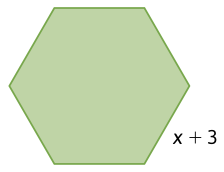
\includegraphics[width=0.25\textwidth]{../images/20230319032932}
    \caption{}
    \label{fig:20230319032932}
\end{figure}

\begin{solutionbox}{4cm}
    \begin{multicols}{2}
      Perímetro:
      \begin{align*}
        P & =6(x+3)\\
            & =6x+18
      \end{align*}

      Área:
      \begin{align*}
        A & =\dfrac{nLa}{2}\\
        & =\dfrac{6(x+3)a}{2}\\
        & =3a(x+3)
      \end{align*}

    \end{multicols}
  \end{solutionbox}